% SHA-256 padding [FIPS 180-4, §5.1.1]: the message, a single 1 bit, k zero bits, and the
% message length l as a 64-bit big-endian number, filling a whole number of 512-bit blocks.
% Original drawing for the Hash library.
\documentclass[tikz,border=6pt]{standalone}
\usepackage[T1]{fontenc}
\usepackage{lmodern}
% Shared style for the Hash diagrams.
% Palette: Okabe–Ito (colour-blind safe). Every diagram is drawn on an opaque white card so it
% stays legible on dark page themes.
\usetikzlibrary{arrows.meta,positioning,calc,fit,backgrounds}
\definecolor{hsblue}{HTML}{0072B2}
\definecolor{hsorange}{HTML}{E69F00}
\definecolor{hsgreen}{HTML}{009E73}
\definecolor{hsvermilion}{HTML}{D55E00}
\definecolor{hspurple}{HTML}{CC79A7}
\definecolor{hsink}{HTML}{1F2933}
\tikzset{
  >={Stealth[length=2.2mm]},
  every node/.style={font=\sffamily\small, text=hsink},
  wire/.style={draw=hsink, line width=0.6pt, ->},
  reg/.style={draw=hsink, line width=0.6pt, fill=hsblue!12, minimum width=9mm, minimum height=7mm},
  fn/.style={draw=hsink, line width=0.6pt, fill=hsorange!25, rounded corners=2pt, minimum width=10mm, minimum height=6mm},
  input/.style={draw=hsink, line width=0.6pt, fill=hsgreen!20, minimum width=9mm, minimum height=6mm},
  add/.style={circle, draw=hsink, line width=0.6pt, fill=white, inner sep=0pt, minimum size=5mm, font=\sffamily\bfseries},
  card/.style={fill=white, rounded corners=4pt},
}

\begin{document}
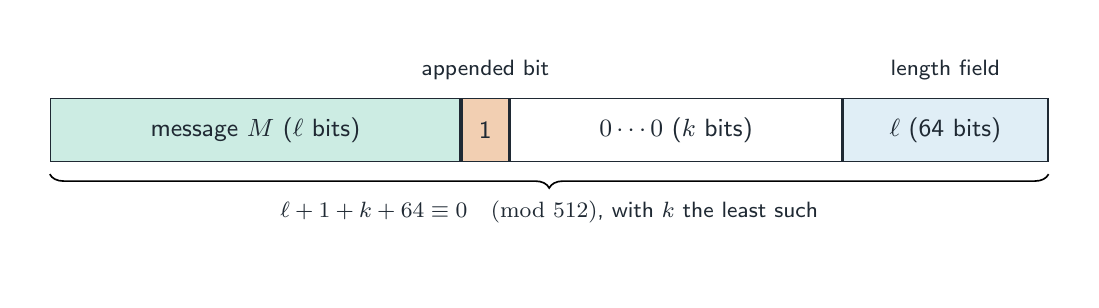
\begin{tikzpicture}[seg/.style={draw=hsink, line width=0.6pt, minimum height=8mm, inner sep=2pt}]
  \node[seg, fill=hsgreen!20, minimum width=52mm, anchor=west] (M) at (0,0) {message $M$ ($\ell$ bits)};
  \node[seg, fill=hsvermilion!30, minimum width=6mm, anchor=west] (one) at (M.east) {1};
  \node[seg, fill=white, minimum width=42mm, anchor=west] (zeros) at (one.east) {$0 \cdots 0$ ($k$ bits)};
  \node[seg, fill=hsblue!12, minimum width=26mm, anchor=west] (len) at (zeros.east) {$\ell$ (64 bits)};
  % Block boundaries.
  \draw[decorate, decoration={brace, amplitude=5pt, mirror}, line width=0.6pt]
    ($(M.south west)+(0,-0.15)$) -- node[below=6pt, font=\sffamily\footnotesize]
    {$\ell + 1 + k + 64 \equiv 0 \pmod{512}$, with $k$ the least such} ($(len.south east)+(0,-0.15)$);
  \node[font=\sffamily\footnotesize, anchor=south] at ($(one.north)+(0,0.1)$) {appended bit};
  \node[font=\sffamily\footnotesize, anchor=south] at ($(len.north)+(0,0.1)$) {length field};
  \begin{scope}[on background layer]
    \node[card, fit=(M)(len), inner sep=8pt, minimum height=3.2cm, yshift=-3mm] {};
  \end{scope}
\end{tikzpicture}
\end{document}
